%!TEX root = ../main.tex

\chapter{System Architecture}
\label{chp:architecture}

As discussed in Chapter \ref{chp:related}, there exist no off-the-shelf solution implementing the \ac{OBDF} paradigm. This implies that for the specific task of dealing with clinical and genomics data, it is necessary to design a system architecture, choosing components in such a way that the whole architecture results in being solid, privacy-oriented (with strong logging capabilities), and being capable to manage genomics data.
This chapter will firstly discuss the overall proposed architecture, that retraces the one presented in previous chapters. Subsequently, each layer will be presented in details, outlining how each components have been configured, reporting eventual code snippets. In order to better describe the source heterogeneity of data that may occur in contexts such as clinical and genomics, available relational data have been distributed among different sources.

\section{System Architecture Design}
\begin{figure}[ht]
    \centering
    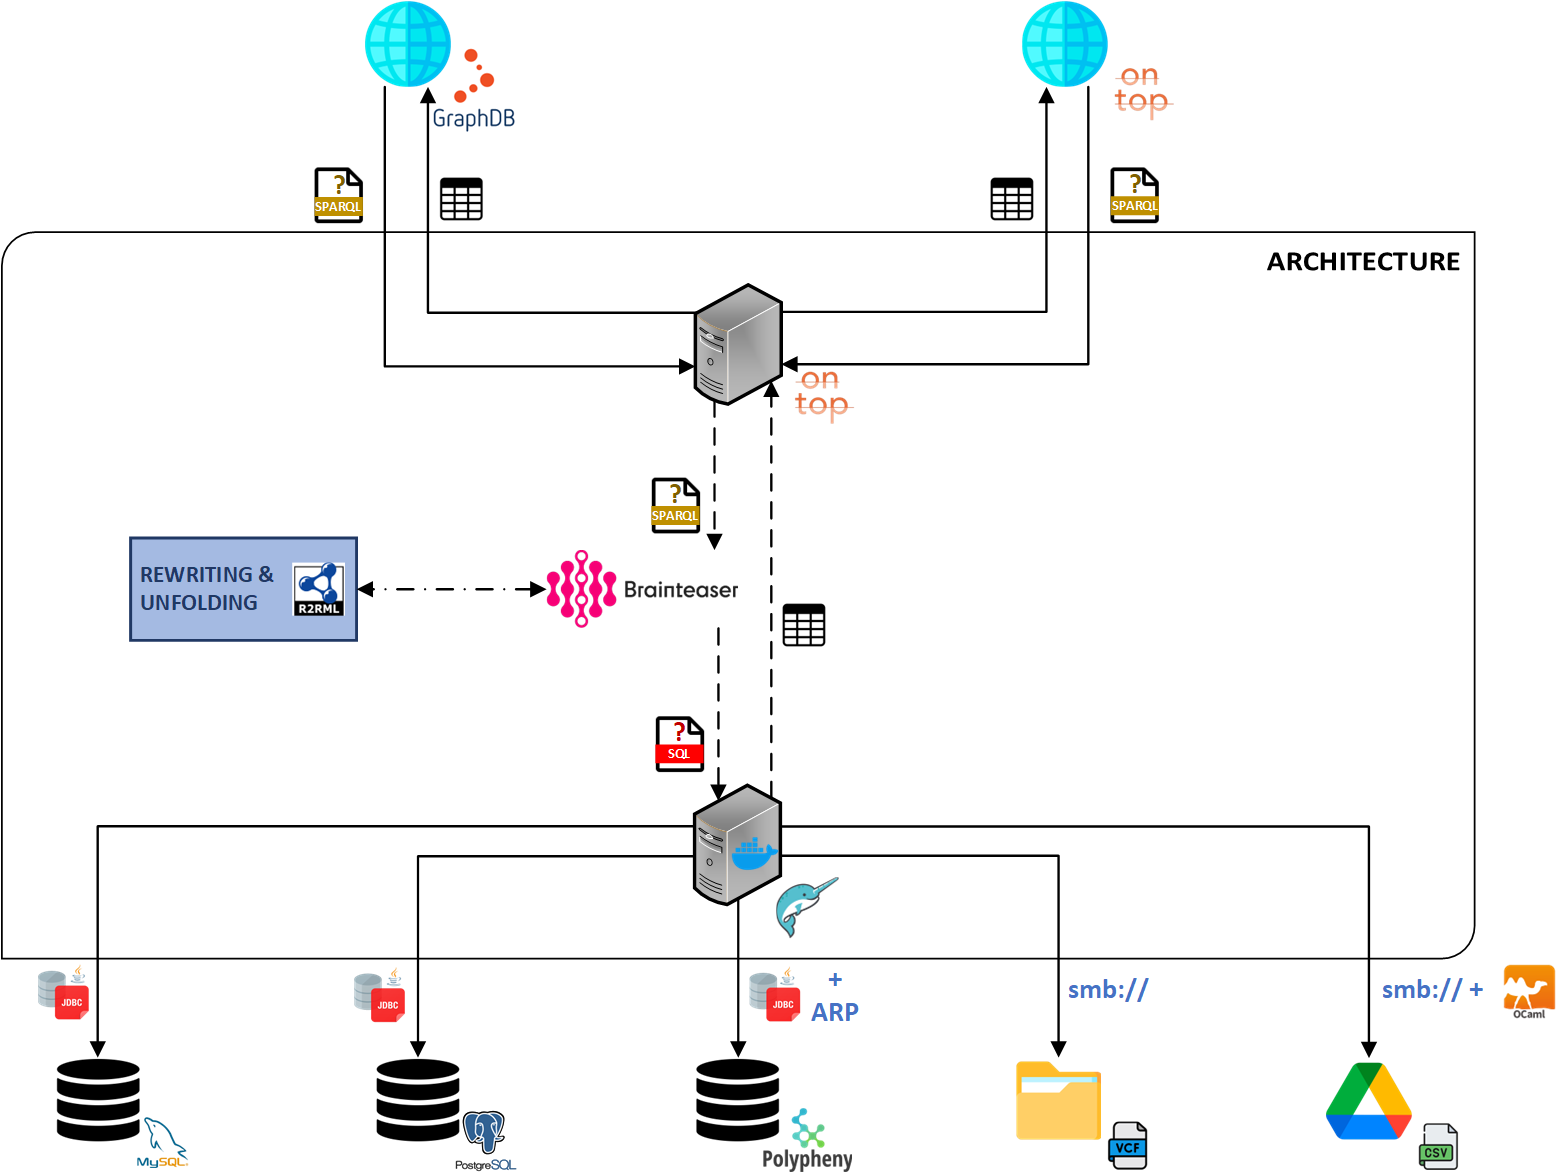
\includegraphics[width=15cm]{res/Drawing1.png}
    \caption{Proposed System Architecture}
    \label{fig:mirco_arch}
\end{figure}
The proposed architecture described in Fig. \ref{fig:mirco_arch} implements the \ac{OBDF} framework. It adopts Ontop as its semantic data integration layer and Dremio as its data federation layer. 

Briefly, Ontop have been chosen because it natively supports two high level mapping languages, that gives more freedom on their optimization, without the need to appeal to low level \ac{DL} languages, it is open-source and well maintained by the Free University of Bolzano data integration team, it comes embedded in GraphDB that offers solid \ac{API}s, and it comes even with an embedded web endpoint.

Dremio have been chosen as the virtualization and federation layer because, as discussed in the Chapter \ref{chp:background}, it is an open-source, robust and scalable software influenced both from its enterprise nature and from a consistent community providing contributions. Moreover, within its installation methods, it is possible to set it up through a Docker image: this may set the basis for the architecture packaging, expanding the image to other software components.

The semantic integration requires an ontology well describing the domain of clinical and genomics data. Considering the reusability principle that stands at the basis of the semantic web, we identified the Brainteaser ontology\footnote{https://brainteaser.dei.unipd.it/ontology/} as suitable for accomplishing this task. 

\section{Data Sources}
Given the relational nature of available data, we distributed it among five different platforms, so to exploit the federation capabilities of the data federation layer. The choice of the sources has been guided also by surveying commonly used ones in the biomedicine field in contexts like research and hospital diagnostic. As we will discuss, they encompasses more structured \ac{DBMS}s as well as simple \ac{CSV} files. We also included a novel \ac{DBMS} system, so to investigate how new, unknown data sources can be federated as soon as they figure out.

\subsection{MySQL}
MySQL\footnote{https://www.mysql.com/it/} is one of the most widely used relational \ac{DBMS} (DBMS) in the world. It is a \ac{FOSS} solution now distributed by Oracle\footnote{https://www.oracle.com/it/}. It is extensively employed across a variety of applications, from small personal projects to critical enterprise environments. In our system architecture, we've chosen MySQL considering its extensive adoption, possibly also in application softwares used in clinics and hospitals to collect patients data. 
In our environment, MySQL's role is to store part of the structured clinical data presented in Chapter \ref{chp:context}. 
The interfacing between MySQL and our data federation layer, Dremio, is performed through MySQL's JDBC connector. This setup allows Dremio to access and query MySQL data seamlessly.
No special modifications or configurations were required to integrate MySQL with Dremio, thanks to Dremio's native support for MySQL. We simply established a new data source within Dremio by specifying the connection parameters.

\subsection{PostgreSQL}
PostgreSQL\footnote{https://www.postgresql.org/} stands out as a widely adopted open-source relational \ac{DBMS}. It is particularly adopted within the research community due to its robustness, advanced features, and strong compliance with SQL standards. Many research institutions and academics prefer PostgreSQL for its extensive capabilities in managing complex data types and its support for sophisticated data manipulation operations. We considered PostgreSQL eligible to be a data source due to its common adoption in research contexts as a data collector.
Again, PostgreSQL's role in our environment is to store another portion of the structured clinical data presented in Chapter \ref{chp:context}.
Just like with MySQL, integrating PostgreSQL with Dremio did not require any specific modifications or additional configurations.

\subsection{Polypheny}
Polypheny \cite{DBLP:conf/bigdataconf/VogtSS18} is an open-source polystore system designed to support diverse data models including relational, document, and graph data. It is engineered to handle mixed workloads and various query languages, making it a versatile platform suitable for dynamic data environments.
In our architecture, we consider Polypheny not just as a standalone polystore but as a potential low-level federator under our main data federation layer managed by Dremio. This perspective is particularly useful because it allows us to leverage Polypheny's ability to handle multiple data models, thus enriching the flexibility and capability of our overall data management system.

\subsubsection{Custom ARP Connector Development}
Unlike the straightforward integrations with MySQL and PostgreSQL, incorporating Polypheny required a more sophisticated approach. We performed this task not only to include Polypheny as one of our data sources but also as a proof of concept about the actual possibility of developing custom ARP connectors.
Dremio's Advanced Relational Pushdown (ARP) framework offers a powerful mechanism to extend Dremio's capability to interact with various data sources by intefacing Dremio's internal query representations into the native query language of the target data source.
For Polypheny, we developed a custom ARP connector to ensure interaction between Dremio and Polypheny. The connector we developed is open-source and available for the community, which can be found at our GitHub repository \footnote{https://github.com/mircocazzaro/dremio-polypheny-arp}.
These connectors rely on the target source having a \ac{JDBC} driver and accepting SQL as a query language, so to have an interface to dialog with.

\subsubsection{Connector implementation Details}
The custom ARP connector was implemented to translate SQL queries from Dremio into the query formats that Polypheny can execute directly.
The ARP plugin template\footnote{https://github.com/dremio-hub/dremio-sqllite-connector} consists of a Java Maven project, that has to be compiled, packed within a \ac{JAR} file and injected, together with the target source \ac{JDBC} driver, into the running Dremio instance.
To customize the template, two files needs to be customize: the storage plugin configuration, which is a Java class \ref{lst:polypheny-arp}, and the plugin ARP file, which is a YAML\footnote{https://yaml.org/} file.
The storage plugin configuration file tells Dremio what the name of the plugin should be, what connection options should be displayed in the source UI, what the name of the ARP file is, which JDBC driver to use and how to make a connection to the JDBC driver.
The ARP YAML file is what is used to modify the SQL queries that are sent to the JDBC driver, allowing you to specify support for different data types and functions, as well as rewrite them if tweaks need to be made for your specific data source. 

\begin{lstlisting}[language=JAVA, caption={The storage plugin configuration file}, label={lst:polypheny-arp}]
/* ... */

@SourceType(value = "POLYPHENY", label = "POLYPHENY")
public class PolyphenyConf extends AbstractArpConf<PolyphenyConf> {
  private static final String ARP_FILENAME = "arp/implementation/polypheny-arp.yaml";
  private static final ArpDialect ARP_DIALECT =
      AbstractArpConf.loadArpFile(ARP_FILENAME, (ArpDialect::new));
  private static final String DRIVER = "org.polypheny.jdbc.Driver";

  @NotBlank
  @Tag(1)
  @DisplayMetadata(label = "Polypheny host <HOST:PORT>")
  public String database;

  /* ... */

  @Tag(2)
  @DisplayMetadata(label = "Record fetch size")
  @NotMetadataImpacting
  public int fetchSize = 200;

  @Tag(6)
  @DisplayMetadata(label = "Polypheny User Name")
  public String username = "pa";

  @Tag(7)
  @DisplayMetadata(label = "Polypheny Password")
  public String password = "";

  @Tag(4)
  @DisplayMetadata(label = "Maximum idle connections")
  @NotMetadataImpacting
  public int maxIdleConns = 8;

  @Tag(5)
  @DisplayMetadata(label = "Connection idle time (s)")
  @NotMetadataImpacting
  public int idleTimeSec = 60;

  @VisibleForTesting
  public String toJdbcConnectionString() {
    final String database = checkNotNull(this.database, "Missing database.");

    return String.format("jdbc:polypheny://%s", database);
  }


  private CloseableDataSource newDataSource() {
    return DataSources.newGenericConnectionPoolDataSource(DRIVER,
      toJdbcConnectionString(), username, password, null, DataSources.CommitMode.DRIVER_SPECIFIED_COMMIT_MODE,
            maxIdleConns, idleTimeSec);
  }
}
\end{lstlisting}

With respect to the storage plugin configuration Java class \ref{lst:polypheny-arp}, being Polypheny still an embryonic project not allowing for user management, but rather having a default user "pa" with empty password, fields are pre-filled with default values. The class specification is then interpreted at run time from Dremio, setting up a form with input fields corresponding to each @DisplayMetadata annotation.
The DRIVER static and immutable variable contains the class path of the Polypheny \ac{JDBC} driver. The newDataSource() method is invoked at form submission, setting up the connection to the Polypheny instance.

\subsection{NAS Folders}
Dremio offers native support for a variety of "relational" file types such as \ac{CSV}, Excel, \ac{JSON}, and \ac{VCF}. These files may be physically moved within the Dremio instance, but losing any streaming capability, or by attaching a \ac{NAS} source to it. In fact, Dremio integrates a connector to local folders, reading supported files within them. The name \ac{NAS} on this typology of data source is ambiguous: the term refers to storage units usually located within the same \ac{LAN} of one or more hosts accessing it, while in Dremio is used to generically refer to a folder to which it can access.
This in practice means Dremio can browse local folders: thus, if NAS shared folders are mounted within the Dremio server through the \ac{SMB} protocol, they can be browsed as well.
In Linux environments where the standalone version of Dremio is used, its daemon must have permission to read these folders; in environments where the Docker image is employed, where a clear separation between the host file system and the Docker context occurs, folders and \ac{NAS} shares must be mapped. This is obtained with Docker Volumes\footnote{ https://docs.docker.com/storage/volumes/}, and in particular the “Host Volume” paradigm.
\begin{lstlisting}[language=bash, caption={Docker command to run a Dremio container with a Host Volume}, label={lst:docker-host-volume}]
$ docker run -v NAS_PATH/folder:/opt/dremio/folder -p 9047:9047 -p 31010:31010 -p 45678:45678 -p 32010:32010 --name hereditary_dremio dremio/dremio-oss
\end{lstlisting}
For the purposes of our project, we have utilized the \ac{NAS} data source to store a portion of our genomics data. Specifically, we have chosen to include data in \ac{VCF} files. \ac{VCF} is a text file format generally used in bioinformatics for storing gene sequence variations.

\subsection{Google Drive}
Google Drive is a widely used cloud storage service offered by Google that allows users to save files and access them from any device connected to the internet. Users can store documents, spreadsheets, and presentations, collaborate with others, and have all their work backed up safely.
We chose to consider Google Drive as a data source for our system architecture primarily because of its widespread use in various contexts, including scenarios where Google Sheets are frequently adopted for data collection and management. Google Sheets, part of the Google Drive suite, is particularly popular in both academic and industrial settings for its ease of use and collaborative features.
The approach to integrating Google Drive is identical to that of the \ac{NAS} system, as long as Google Drive is adapted to a local host folder. This adaptation allows Dremio to interact with Google Drive as if it were interacting with local file systems, thereby simplifying access and manipulation of data stored in Google Drive.
The adaptation of Google Drive to a local system is facilitated by a tool known as google-drive-ocamlfuse\footnote{https://github.com/astrada/google-drive-ocamlfuse}, which provides a FUSE-based file system backed by Google Drive. This tool was built using OCaml, a functional programming language known for its expressiveness, efficiency, and robustness. OCaml is utilized to handle the logical operations and data structure management, ensuring that the application runs efficiently and securely. \ac{FUSE} is a software interface for Unix-like computer operating systems that lets non-privileged users create their own file systems without editing kernel code. This is used in google-drive-ocamlfuse to mount Google Drive as a file system on the user's computer.
\subsubsection{Adaptation of Google Sheets}
With the google-drive-ocamlfuse tool, Google Sheets can be adapted to local Excel files, which are natively supported by Dremio. This adaptation is crucial because it allows Dremio to perform operations on Google Sheets just as it would on local Excel files, enabling seamless data processing and integration without needing to convert or move data physically.
\subsubsection{Configuration and Usage}
Configuring google-drive-ocamlfuse involves setting up Google Drive as a mounted file system. Once mounted, the Google Drive folder behaves like any other directory on the local system.
\begin{lstlisting}[language=bash, caption={google-drive-ocamlfuse Tool installation procedure}, label={lst:ocamlfuse}]
# Installation of google-drive-ocamlfuse
$ sudo add-apt-repository ppa:alessandro-strada/ppa
$ sudo apt-get update
$ sudo apt-get install google-drive-ocamlfuse

# Authentication and mounting
$ google-drive-ocamlfuse
$ mkdir ~/google-drive
$ google-drive-ocamlfuse ~/google-drive
\end{lstlisting}
We used the Google Drive data source to store the remaining part of \ac{VCF} genomics data.


\section{Federation and Virtualization Layer}
At the bottom of our system architecture we do have a software component that encompasses both the federation and virtualization functionalities. In fact, this component not only allows to seamlessly connecting to multiple diverse data sources, but also serves as a virtualizator by creating unmaterialized virtual views of the integrated data. This dual functionality is essential in our scenario for efficiently managing data access and manipulation across the disparate systems involved in our project.
\subsection{Role of Federator}
As a federator, this layer allows for extensive connectivity, facilitating interactions with various types of data sources ranging from traditional relational databases like MySQL and PostgreSQL to modern polystore systems such as Polypheny, and even cloud-based storage solutions like Google Drive. The ability to federate across these diverse sources means that data, regardless of where it is stored or in what format, can be accessed and queried as if it were located within a single, homogeneous database.
\subsection{Role of Virtualizator}
On the virtualization side, the layer enables the creation of virtual views that do not require materialization. These views treats relations exposed from underlying data sources as if they are actual tables within the same database schema: as Fig. \ref{fig:virtual} shows, this implies that these tables can be joined together and thus expose the most meaningful information to the upper architecture layers. Moreover, tables can be joined with pre-defined views, further enhancing the virtualization capabilities. No data is physically stored within this layer, but rather queries coming into this layer are dynamically interpreted and delegated to the source \ac{DBMS}s. This approach ensures that the most current data is always presented to the user or application, without the overhead and delay associated with physical data integration. In the subsequent sections, a diagram will be included to illustrate how these virtual views are structured and managed within our system.
\begin{figure}[ht]
    \centering
    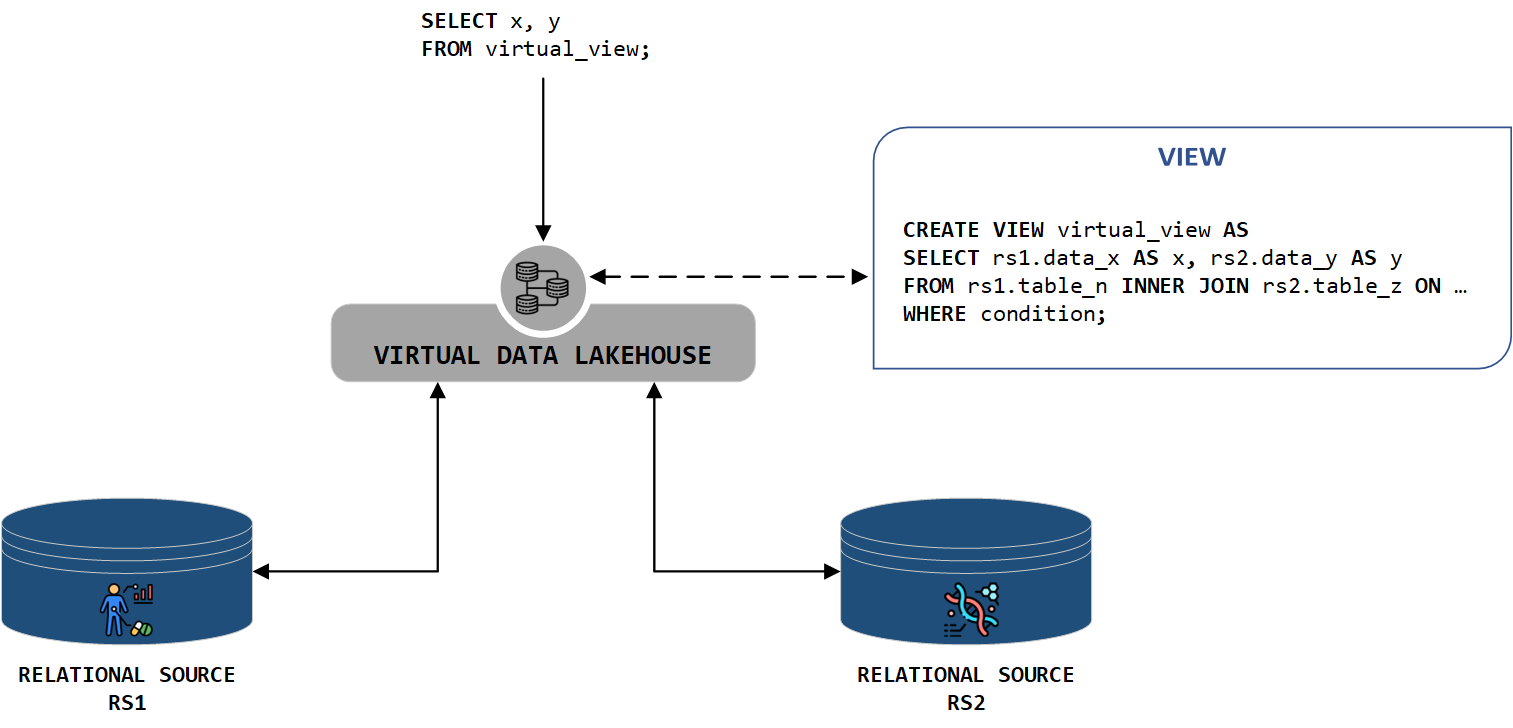
\includegraphics[width=15cm]{res/Drawing2.png}
    \caption{Virtual Views}
    \label{fig:virtual}
\end{figure}
\subsection{Focus on Dremio}
\subsubsection{Web Interface}
One of the main features of Dremio is its user-friendly web interface, which provides a graphical user interface (\ac{GUI}) that simplifies the process of data management. This interface is particularly beneficial for defining and managing virtual views. As shown in Fig. \ref{fig:screenshot} users can interact with the system through the web interface to run queries, visualize query results and configure the system settings.
\subsubsection{Defining Virtual Views}
Within Dremio's web interface, users can create and manage virtual views. These datasets do not store any data themselves but instead provide a virtual schema on top of physical data stored across different sources. Users can define virtual views by writing standard SQL queries that join, filter, or transform the data across these sources. For instance, a researcher might join genomic data stored in a NAS system with patient data from a MySQL database to analyze correlations between genetic markers and health outcomes.
\subsubsection{JDBC Connection}
Apart from its web interface, Dremio also supports \ac{JDBC} connections, allowing it to integrate seamlessly with a variety of programming environments and data tools. This \ac{JDBC} support is crucial for automating data processes and integrating with other applications that require programmatic access to the data federation layer. Developers can use the \ac{JDBC} driver to connect directly to Dremio from their applications, enabling them to run queries programmatically and retrieve data for further processing or analysis. This capability is essential for building automated data pipelines and for applications that need to interact dynamically with the data layer.

\section{Ontology Layer: Brainteaser Ontology}
In our system architecture, the ontology layer is essential in modeling and managing the complex relationships between genomics data interlaced with clinical values and patients' medical records. Through an extensive review of the literature and existing resources, we identified a suitable ontology that effectively encapsulates these intricate data relationships: the Brainteaser Ontology.
\subsection{Brainteaser Ontology Overview}
Represented in Fig. \ref{fig:bto}, the Brainteaser Ontology is specifically designed to model the multifaceted context of genomics and clinical data. This ontology provides a structured framework that facilitates the integration of diverse data types, ranging from detailed genomic sequences to comprehensive patient medical records. By adopting this ontology within our system, we can link data across these varied domains effectively, exploiting all the potentials discussed in the background analysis, and enhancing our ability to conduct meaningful analytical analyses that require a deep understanding of both genetic and clinical factors.
The ontology is part of the broader Brainteaser project, which aims to address complex biomedical challenges through innovative data integration techniques and advanced computational models. More information about the Brainteaser project and its initiatives can be found on the official website\footnote{https://brainteaser.dei.unipd.it/ontology/}.
\begin{figure}[ht]
  \centering
  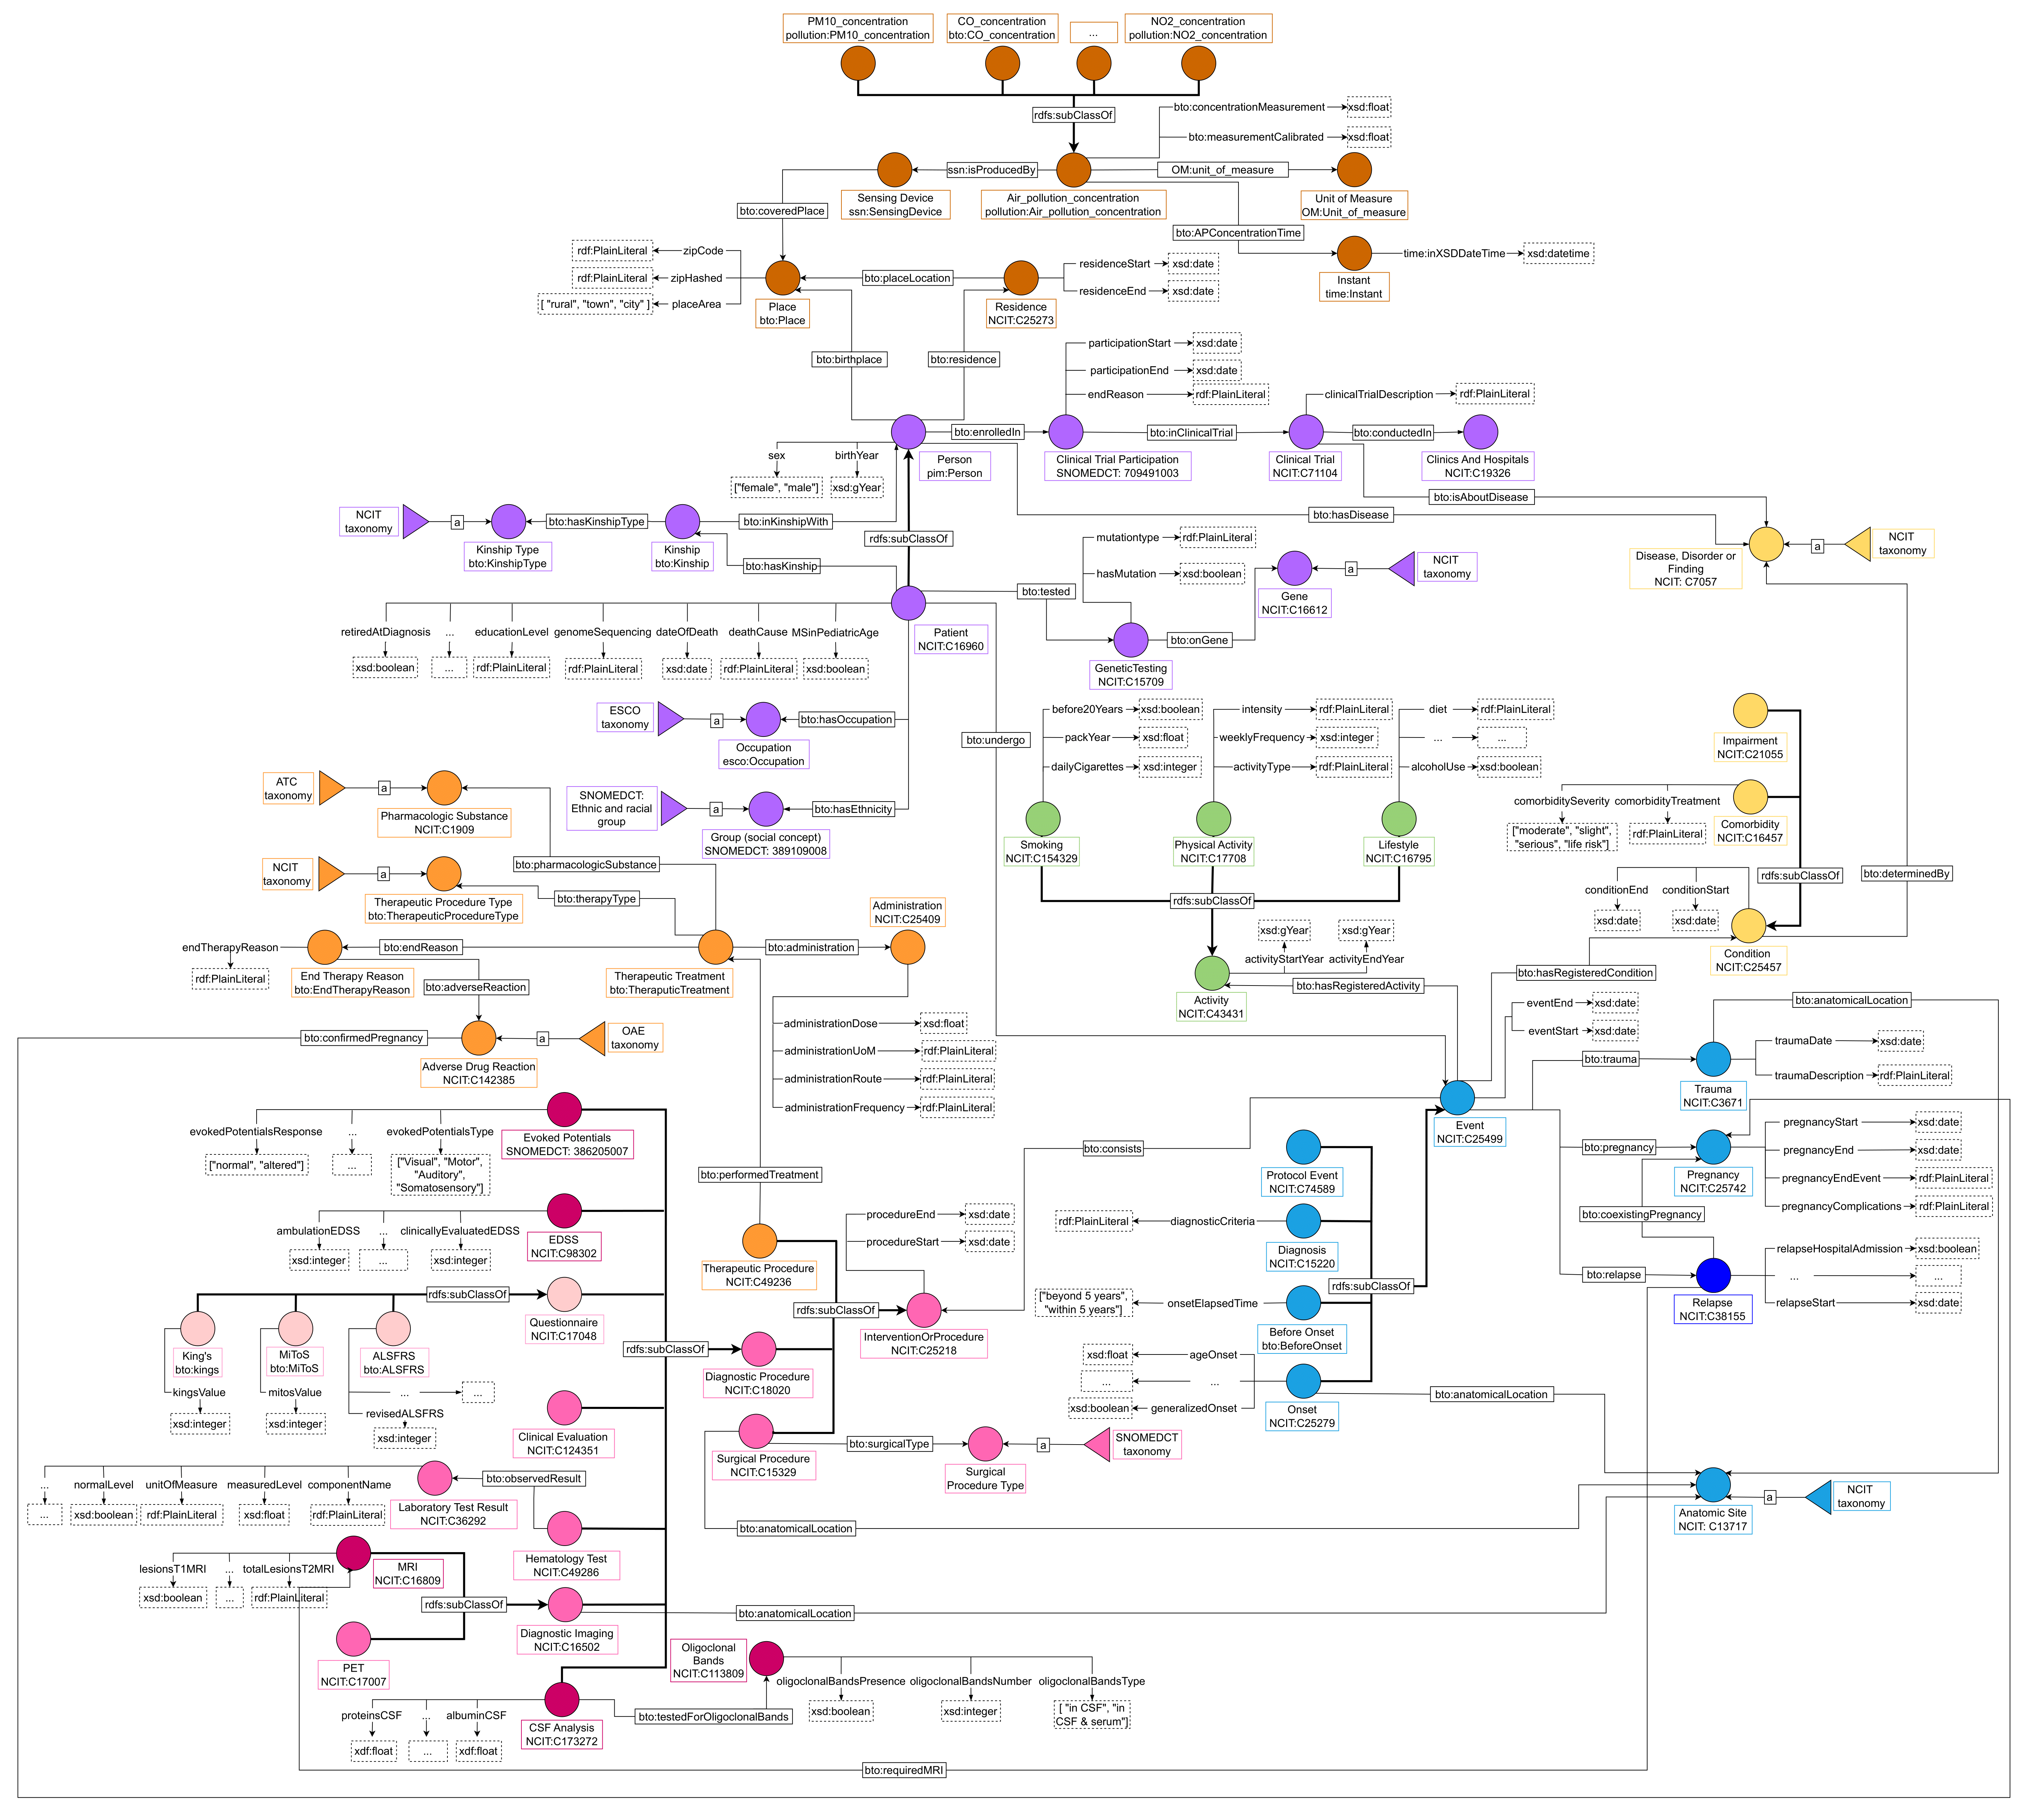
\includegraphics[width=15cm]{res/brainteaser.png}
  \caption{The Brainteaser Ontology}
  \label{fig:bto}
\end{figure}
\subsection{Ontology Features and Capabilities}
The Brainteaser Ontology models meticulously various aspects of patient health data, including genetic markers, clinical symptoms, diagnostic test results, and treatment responses. This comprehensive modeling approach ensures that all relevant data dimensions are captured and can be queried effectively. One of the key strengths of the Brainteaser Ontology is its focus on interoperability. It is built to integrate seamlessly with existing medical and genomic data standards, facilitating easy data exchange and compatibility with other health information systems. As new discoveries are made and healthcare practices evolve, the ontology is structured to be scalable and flexible. It can accommodate additional data types and relationships, supporting the ongoing growth and diversification of biomedical data.
\subsection{Ontology Implementation}
In our system, the Brainteaser Ontology acts as the vocabulary for designing semantic queries over data. By mapping our virtual data model with this ontology, we ensure that data from disparate sources can be integrated coherently and that complex queries involves all data coming from the heterogeneous data sources.

\section{OBDA Layer}
In our architecture, The component realizing the \ac{OBDA} paradigm, that aims to set up a \ac{VKG}, is Ontop.
Ontop comes in different shapes: different tools are provided for accomplishing different tasks.
In this section we will discuss the different Ontop tools that have been employed in our project alongside their actual role, with also code examples.
\subsection{Ontop Mapping}
Protégé is a well-known tool for ontology modelling, developed and maintained by the Stanford University. Apart from its standard capabilities, it is open to custom plugins that can be installed on demand, that expand its features.
To develop ontology mappings between an ontology and a single relational data source, as in the \ac{OBDA} paradigm is defined, the Ontop Mappings plugin for Protégé have been realized. Its utilization process is defined as follows:
\begin{itemize}
  \item The ontology that has to be mapped has to be opened with Protégé;
  \item The Ontop Mappings plugin has three tabs: the first one is about setting up the \ac{JDBC} connection with the relational source (i.e. Dremio). The \ac{JDBC} driver has to be manually loaded within the Protégé "connectors" folder;
  \item The second tab is about defining Ontop properties. For the mapping task, no specific property needs to be defined;
  \item The third tab is the mappings editor. Here, there are two different input fields: one asks for a portion of the graph, in Turtle notation, with autocomplete features; the second one is about the SQL query against the relational sources. Rows coming from the relational sources are directly mapped by including fields name within curly brackets in the Turtle syntax. Note that if there are mistakes in the Turtle notation (e.g. the subgraph doesn't match with the ontology), the mapping can't be added.
  \item After defining all mappings, they can be validated by clicking on "Validate". \ac{SQL} queries are executed and if they are wrong, or field names doesn't coincide with the one defined within curly brackets, an exception is raised;
  \item By saving the Protégé project, an .obda file is created in the ontology folder, containing mappings definition.
\end{itemize}  

For shortness, a portion of the mappings implementation between the virtual relational schema exposed by Dremio and the Brainteaser Ontology is shown in Code \ref{lst:mappings}.

\begin{lstlisting}[language=OntopNative, caption={Mappings definition between the virtual relational schema exposed by Dremio and the Brainteaser Ontology}, label={lst:mappings}]
  [MappingDeclaration] @collection [[
  mappingId	MAPID-5b34961b80264140bb779dbd296424ac
  target		bto:Patient{patient} a bto:Patient . 
  source		SELECT patient FROM "@mirco.cazzaro"."STATIC_VARS";

  mappingId	MAPID-f24debb89dc84f73a47acdf763ec0b4f
  target		bto:Patient{patient} bto:alive {alive}^^xsd:boolean . 
  source		SELECT patient, LCASE(alive) AS alive
        FROM "@mirco.cazzaro"."STATIC_VARS"
        WHERE alive <> '';

  mappingId	MAPID-5b2c0dfea75d44279ce8ddde95f2a9aa
  target		bto:Patient{patient} bto:sex {sex}^^xsd:string . 
  source		SELECT patient, LCASE(sex) AS sex
        FROM "@mirco.cazzaro"."STATIC_VARS"
        WHERE sex <> '';

  mappingId	MAPID-51a6eb8de7c64b7bbe4fe62d8188208c
  target		bto:Patient{patient} bto:undergo bto:eventOnset1{patient} . bto:eventOnset1{patient} a bto:Onset ; bto:eventStart {onsetDate}^^xsd:datetime ; bto:bulbarOnset {onset_bulbar}^^xsd:boolean ; bto:axialOnset {onset_axial}^^xsd:boolean ; bto:generalizedOnset {onset_generalized}^^xsd:boolean ; bto:limbsOnset {onset_limbs}^^xsd:boolean . 
  source		SELECT patient, onsetDate, LCASE(onset_bulbar) AS onset_bulbar, LCASE(onset_axial) AS onset_axial, LCASE(onset_generalized) AS onset_generalized, LCASE(onset_limbs) AS onset_limbs FROM "@mirco.cazzaro"."STATIC_VARS";

  mappingId	MAPID-541428e7a83441f5bd29e52d66ffc52e
  target		bto:Patient{patient} bto:undergo bto:eventOnset2{patient} . bto:eventOnset2{patient} a bto:Onset ; bto:ageOnset {age_onset}^^xsd:float . 
  source		SELECT patient, age_onset FROM "@mirco.cazzaro"."STATIC_VARS" WHERE age_onset <> '';

  mappingId	MAPID-ff2b4bdc90af468793b4f58105fa555f
  target		bto:Patient{patient} bto:undergo bto:diagnosis{patient} . bto:diagnosis{patient} a bto:Diagnosis ; bto:eventStart {diagnosisDate}^^xsd:datetime . 
  source		SELECT patient, diagnosisDate FROM "@mirco.cazzaro"."STATIC_VARS";

  mappingId	MAPID-13ab39d8b67c4f34a206b7f4bcc1f442
  target		bto:Patient{patient} bto:hasEthnicity bto:eth{patient} . bto:eth{patient} rdfs:label {ethnicity}@en . 
  source		SELECT patient, ethnicity FROM "@mirco.cazzaro"."STATIC_VARS" WHERE ethnicity <> '';

  mappingId	MAPID-56da0e23dc6b4cb3a0bfc475f4bcb65f
  target		bto:eventOnset3{patient} bto:anatomicalLocation bto:location{patient} . bto:location{patient} rdfs:label {onset_location}^^xsd:string . 
  source		SELECT patient, onset_location FROM "@mirco.cazzaro"."STATIC_VARS" WHERE onset_location <> '';

  mappingId	MAPID-5ea1e8edbbb1446fb50e887c4f0605dd
  target		bto:eventOnset4{patient} bto:consists bto:clinicalEvaluation{patient} . bto:clinicalEvaluation{patient} a bto:ClinicalEvaluation ; bto:predominantLimbsSide {onset_limbs_side}^^xsd:string ; bto:predominantLimbsImpairment {onset_limbs_impairment}^^xsd:string . 
  source		SELECT patient, onset_limbs_side, onset_limbs_impairment
        FROM "@mirco.cazzaro"."STATIC_VARS"
        WHERE onset_limbs_side <> '' OR onset_limbs_impairment <> '';
  ]]
\end{lstlisting}

\subsection{Ontop SPARQL}
The aim of the OBDA approach is executing \ac{SPARQL} queries over a \ac{VKG}. Testing mapping correctness before their utilization in a running environment is essential. The Ontop SPARQL plugin for Protégé accomplishes this task. Given its role of a testing tool, it allows to analyze the "\ac{SQL} translation" of the running \ac{SPARQL} query.
\subsection{Ontop Endpoint}
The Ontop Standalone Endpoint provides a server environment where Ontop can operate independently, offering both an API and a web interface for running SPARQL queries over the virtual knowledge graph. This setup is particularly useful for environments where integration with existing data management systems is necessary, as it comes as an independent and lightweight tool.
\subsection{Ontop with GraphDB}
Integrating Ontop with GraphDB leverages the strengths of both platforms, combining Ontop's powerful OBDA capabilities with GraphDB's management functionalities. GraphDB allows to manage simultaneously different graph databases, where data is collected in independent "repositories". In particular, repositories can be standard repositories, thus ingesting \ac{RDF} data, or virtual, that actually is an adaptation of the repository over an Ontop instance. This solution is particularly indicated for those scenarios where an easy-to-use web interface is necessary, allowing to export retrieved data in various formats.